\section{Fraseio}
\label{sec:fraseio}
\index{Música!Fraseio}

O fraseio (frasear) na composição musical, implica  tornar clara e identificável, 
pelo uso adequado de acentuações e cadencias, 
o inicio e o final das \hyperref[sec:Frase]{\textbf{frases}} numa peça musical \cite[pp. 336]{medteoria} \cite[pp. 19]{holst1998abc}.
Anteriormente, 
o fraseio na música era deixado para ser escolhido livremente, pelo sentido de bom senso e gosto de cada intérprete;
porém, atualmente é comum que os compositores modernos usem vários simbolos para indicar o fraseio \cite[pp. 348]{stainer2009dictionary}.
Assim, as frases são separadas na pauta usando signos como a \hyperref[fig:Cesura]{\textbf{cesura}}\footnote{Para
 mais detalhes ir a Pagina \pageref{fig:Cesura}.}  \cite[pp. 668]{apel1969harvard},
que servem para que o interprete recupere o folego 
para  a seguinte frase musical \cite[pp. 18]{holst1998abc} \cite[pp. 48]{howard1991aprendendo},
da mesma forma que acontece com o signos de pontuação na leitura de um discurso.




\begin{figure}[!h]
\begin{elaboracion}{Cesura}
\index{Música!Cesura}
A cesura é um simbolo que indica uma pequena pausa entre duas frases,
é equivalente a dizer que a ultima nota da primeira frase terá uma diminuição pequena, só para pegar folego;
entre os símbolos usados para a cesura temos a virgula ``\textbf{,}'' 
ou também uma ``\textbf{v}'', ou ``\textbf{//}'', ou ``\textbf{/}'' 
\cite[pp. 252]{medteoria} \cite[pp. 18]{holst1998abc}.
A seguinte figura mostra o uso da cesura, onde é indicado que o interprete deverá 
dar uma pausa na ultima nota da primeira frase, neste caso diminuindo a duração da nota sol.\\
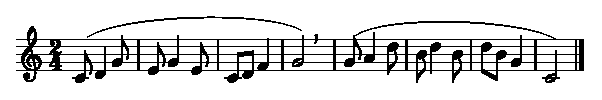
\includegraphics[width=\textwidth]{chapters/cap-musica-topicos/cesura1-1.eps}
\end{elaboracion}
\label{fig:Cesura}
\end{figure}
 
Por outra lado, para os executantes da música, 
o fraseamento é a arte de interpretar as frases individuais ou elas em conjunto, numa composição musical;
sendo este ponto, 
uma caraterística importante da estética particular que dá cada interprete à música 
\cite[pp. 257]{medteoria} \cite[pp. 624]{latham2008diccionario}.
Falando em termos mais rigorosos, 
o fraseado na interpretação refere-se à separação de uma melodia na suas frases constituintes 
\cite[pp. 668]{apel1969harvard}.

Uma caraterística interessante da música, 
é que o comprimento das frases é afetado diretamente pela capacidade respiratória do ser humano,
mesmo em instrumentos que não são de sopro como o piano \cite[pp. 48]{howard1991aprendendo},
isto poderia dever-se a que nos sentimos mais confortáveis de escutar composições musicais,
que relacionamos facilmente com um discurso falado.

\begin{example}
Leia  o seguinte texto respeitando acentos, descansos e signos de admiração e interrogação:
\begin{citando}%%
Boa tarde amigo!\\
Como você está?\\
Bem, muito obrigado.
\end{citando}%%

Agora, com a ajuda de um piano, execute a melodia mostrada na Figura \ref{fig:conversa1},
e tente respeitar o mesmo fraseio que no texto, se ajude usando as ligaduras de expressão e a cesura.
\end{example}

\begin{figure}[!h]
\centering
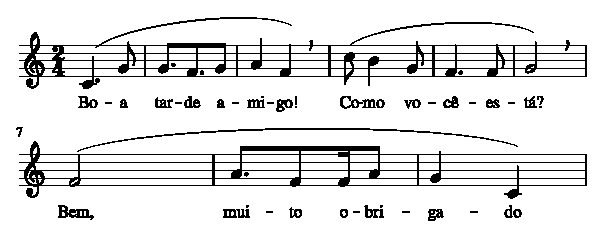
\includegraphics[width=\textwidth]{chapters/cap-musica-topicos/conversa-1.eps}
\caption{Frases musicais.}
\label{fig:conversa1}
\end{figure}

% https://es.wikipedia.org/wiki/Fraseo
% https://en.wikipedia.org/wiki/Musical_phrasing


